\chapter{比較兩組樣本的假說檢定}

    前一章我們介紹了假說檢定的架構,以及如何檢定一組樣本背後的母體平均值(或母體比例)是否大於、等於、或小於我們預想的數值。然而,在生醫研究中,我們更常有興趣的是,從兩個母體各抽出一組樣本後,檢定背後兩個母體的平均值或是比例之間的關係。例如,在血壓藥物的隨機對照實驗中,我們將受試者隨機分為兩組並各給予不同的藥物治療。此時我們有興趣的是,接受兩種藥物治療後的平均血壓是否有差別,進而推論兩種藥物的效果優劣。因此,本章我們將著重探討如何針對兩組樣本的母體平均值(或母體比例)差異作檢定,以及如何為這個差異建構信賴區間。
    
    \begin{introduction}[第 \thechapter 章學習目標]
        \item 在各種母體假設下,利用 $Z$ 及 $t$ 檢定比較兩組樣本的母體平均
        \item 檢定比較兩組樣本的母體比例
        \item 母體平均差值及母體比例差值的信賴區間建構
    \end{introduction}

\section{母體平均的獨立雙樣本檢定:兩個母體均為常態分布且變異數已知}

    我們首先討論如何比較兩組常態樣本背後之母體平均。假設已知兩個母體均服從常態分布且互相獨立。兩者母體平均未知,分別記為 $\mu_1$ 和 $\mu_2$,但變異數均已知,分別為 $\sigma_1^2$ 和 $\sigma_2^2$。若將兩組樣本的樣本平均記為 $\bar{X}_1, \bar{X}_2$,則其抽樣分布應分別為
    \[\bar{X}_1 \sim \NN\Big(\mu_1, \frac{\sigma_1^2}{n_1}\Big) \qquad ; \qquad \bar{X}_2 \sim \NN\Big(\mu_2, \frac{\sigma_2^2}{n_2}\Big)\]
    由於兩組樣本互相獨立,因此兩個樣本平均也互相獨立。將兩個樣本平均相減後,期望值亦為相減,變異數則因獨立而為相加:
    \[\bar{X}_2-\bar{X}_1 \sim \NN \Big(\mu_2 - \mu_1, \frac{\sigma_1^2}{n_1} + \frac{\sigma_2^2}{n_2}\Big)\]
    由於 $\bar{X}_2-\bar{X}_1$ 服從常態分布,我們可以將其做 $z$ 轉換,轉換後即服從標準常態分布
    \[\frac{(\bar{X}_2-\bar{X}_1)-(\mu_2-\mu_1)}{\sqrt{\frac{\sigma_1^2}{n_1} + \frac{\sigma_2^2}{n_2}}} \sim \ZZ\]
    此時根據虛無假說和對立假說的形式,我們可以對 $\mu_2-\mu_1$ 的數值建構檢定。為了簡單起見,我們假定虛無假說都是 $H_0: \mu_2 = \mu_1$ 的形式,也就是在虛無假說下兩個母體的平均相等。如此一來,在虛無假說下,以下 $Z$ 檢定量的虛無分布為標準常態分布:
    \[Z := \frac{\bar{X}_2-\bar{X}_1}{\sqrt{\frac{\sigma_1^2}{n_1} + \frac{\sigma_2^2}{n_2}}} \sim \ZZ\]
    對立假說隨著 $\mu_2-\mu_1$ 的方向不同而決定其為右尾、左尾或雙尾檢定。若設定為 $H_1: \mu_2 > \mu_1$ 則為右尾檢定;若設定為 $H_1: \mu_2 < \mu_1$ 則為左尾檢定;若設定為 $H_1: \mu_2 \ne \mu_1$ 則為雙尾檢定。

    \noindent\underline{\textbf{右尾檢定}}

    右尾檢定的假說形如 $H_0: \; \mu_2 = \mu_1 \; ; \; H_1: \; \mu_2 > \mu_1$。我們可以用 $p$ 值法來建構檢定:當對立假說為真時,$\bar{X}_2 - \bar{X}_1$ 的期望值 $\mu_2 - \mu_1$ 會大於 0,因此 $Z$ 偏大的方向是比較「極端」的方向。根據 $p$ 值的定義可以寫出
    \[p = \PP(\ZZ \ge Z)\]
    此時若 $p \le \alpha$ 則拒絕虛無假說、接受對立假說;反之則無法拒絕虛無假說。同樣地,我們也可以用拒絕域法建構檢定而得到拒絕區為 $Z \ge z_\alpha$,統計量臨界值為 $z_\alpha$。

    \noindent\underline{\textbf{左尾檢定}}

    若假說形如 $H_0: \; \mu_2 = \mu_1 \; ; \; H_1: \; \mu_2 < \mu_1$,我們可以用 $p$ 值法來建構檢定:當對立假說為真時,$\bar{X}_2 - \bar{X}_1$ 的期望值 $\mu_2 - \mu_1$ 會小於 0,因此 $Z$ 偏小的方向是比較「極端」的方向。根據 $p$ 值的定義可以寫出
    \[p = \PP(\ZZ \le Z)\]
    此時若 $p \le \alpha$ 則拒絕虛無假說、接受對立假說;反之則無法拒絕虛無假說。同樣地,我們也可以用拒絕域法建構檢定而得到拒絕區為 $Z \le z_\alpha$,統計量臨界值為 $z_\alpha$。

    \noindent\underline{\textbf{雙尾檢定}}

    若假說形如 $H_0: \; \mu_2 = \mu_1 \; ; \; H_1: \; \mu_2 \ne \mu_1$,我們可以用 $p$ 值法來建構檢定:當對立假說為真時,$\bar{X}_2 - \bar{X}_1$ 的期望值 $\mu_2 - \mu_1$ 會往兩側遠離 0,因此 $Z$ 不論偏大或偏小都是「極端」的方向。且因為 $Z$ 的虛無分布期望值為零,$Z$ 和 $-Z$ 的極端程度是一樣的。因此,根據 $p$ 值的定義可以寫出
    \[p = \PP((\ZZ \ge |Z|)\cup(\ZZ \le -|Z|)) = 2\PP(\ZZ \ge |Z|)\]
    此時若 $p \le \alpha$ 則拒絕虛無假說、接受對立假說;反之則無法拒絕虛無假說。同樣地,我們也可以用拒絕域法建構檢定而得到拒絕區為 $|Z| \ge z_{\alpha/2}$,統計量臨界值為 $\pm z_{\alpha}$ 。

    以下我們用表 \ref{tab:two_sample_z} 來整理母體服從常態分布且變異數已知的母體平均雙樣本檢定。由於此檢定比較了兩組獨立樣本,且是用 $Z$ 檢定統計量來建構,統計量的虛無分布為標準常態分布($\ZZ$),因此此檢定亦稱為\textit{獨立樣本 Z 檢定} (Independent sample Z test) 或\textit{雙樣本 Z 檢定} (Two-sample Z test)。

    \begin{table}[htbp]
        \begin{center}
            \begin{tabular}{ccccc}
                \toprule
                虛無假說($H_0$) & 對立假說($H_1$) & 檢定統計量 & $p$ 值 & 拒絕區\\
                \hline
                \multirow{3}{*}{$\mu_2 = \mu_1$} & $\mu_2 > \mu_1$ & \multirow{3}{*}{$Z = \frac{\bar{X}_2-\bar{X}_1}{\sqrt{\frac{\sigma_1^2}{n_1}+\frac{\sigma_2^2}{n_2}}}$} & $\PP(\ZZ \ge Z)$ & $Z \ge z_{\alpha}$\\
                & $\mu_2 < \mu_1$ & &$\PP(\ZZ \le Z)$&$Z \le -z_{\alpha}$\\
                & $\mu_2 \ne \mu_1$ & &$2\times\PP(\ZZ \ge |Z|)$&$|Z| \ge z_{\alpha/2}$\\
                \bottomrule
            \end{tabular}
            \caption{母體為常態分布且變異數已知的母體平均雙樣本檢定(雙樣本 Z 檢定)\label{tab:two_sample_z}}
        \end{center}
    \end{table}

    除了進行檢定外,我們也可以根據 $\bar{X}_2 - \bar{X}_1$ 作 $z$ 轉換後的抽樣分布,建構母體平均差 $\mu_2 - \mu_1$ 的信賴區間。以 $(1-\alpha) \times 100\%$ 雙尾信賴區間為例,因為 $\frac{(\bar{X}_2-\bar{X}_1)-(\mu_2-\mu_1)}{\sqrt{\frac{\sigma_1^2}{n_1} + \frac{\sigma_2^2}{n_2}}} \sim \ZZ$,
    \[\PP\Bigg(-z_{\alpha/2} < \frac{(\bar{X}_2-\bar{X}_1)-(\mu_2-\mu_1)}{\sqrt{\frac{\sigma_1^2}{n_1} + \frac{\sigma_2^2}{n_2}}} < z_{\alpha/2}\Bigg) = 1-\alpha\]
    \[\PP\Bigg[(\bar{X}_2-\bar{X}_1) - z_{\alpha/2} \sqrt{\frac{\sigma_1^2}{n_1} + \frac{\sigma_2^2}{n_2}} < \mu_2-\mu_1  < (\bar{X}_2-\bar{X}_1) + z_{\alpha/2} \sqrt{\frac{\sigma_1^2}{n_1} + \frac{\sigma_2^2}{n_2}}\Bigg] = 1-\alpha\]
    因此,$\mu_2-\mu_1$ 的 $(1-\alpha) \times 100\%$ \textbf{雙尾}信賴區間即為
    \[\Bigg((\bar{X}_2-\bar{X}_1) - z_{\alpha/2} \sqrt{\frac{\sigma_1^2}{n_1} + \frac{\sigma_2^2}{n_2}},  (\bar{X}_2-\bar{X}_1) + z_{\alpha/2} \sqrt{\frac{\sigma_1^2}{n_1} + \frac{\sigma_2^2}{n_2}}\Bigg)\]
    根據我們上一章有關檢定與信賴區間之間關係的探討,當這個雙尾信賴區間未覆蓋到 $0$ 時,等同於在顯著水準 $\alpha$ 下拒絕 $\mu_2 - \mu_1 = 0$ 的虛無假說,並接受 $\mu_2 \ne \mu_1$ 的\textbf{雙尾}對立假說。同理,$\mu_2-\mu_1$ 的 $(1-\alpha) \times 100\%$ 右尾及左尾信賴區間分別為
    \[\Bigg((\bar{X}_2-\bar{X}_1) - z_{\alpha} \sqrt{\frac{\sigma_1^2}{n_1} + \frac{\sigma_2^2}{n_2}}, \infty \Bigg) \quad ; \quad \Bigg(-\infty, (\bar{X}_2-\bar{X}_1) + z_{\alpha} \sqrt{\frac{\sigma_1^2}{n_1} + \frac{\sigma_2^2}{n_2}} \Bigg)\]
    前者未覆蓋到 $0$ 則可接受 $\mu_2 > \mu_1$ 的對立假說,後者未覆蓋到 $0$ 則可接受 $\mu_2 < \mu_1$ 的對立假說。
    
\section{母體平均的獨立雙樣本檢定:兩個母體均為常態分布但變異數未知}

    上一節我們假設了兩個母體均為常態分布且變異數均已知,因此可以將樣本平均的差 $\bar{X}_2-\bar{X}_1$ 進行 $z$ 轉換,且得到在兩母體平均相等($H_0: \mu_1 = \mu_0$)的虛無假說下
    \[Z := \frac{\bar{X}_2-\bar{X}_1}{\sqrt{\frac{\sigma_1^2}{n_1} + \frac{\sigma_2^2}{n_2}}} \sim \ZZ\]
    當變異數未知時,$\sigma_1^2$ 和 $\sigma_2^2$ 均為未知數,因此無法計算 $Z$ 統計量。此時,按照我們之前在單樣本檢定的經驗,我們會希望能以兩組的樣本變異數 $s_1^2$ 和 $s_2^2$ 帶入 $\sigma_1^2$ 和 $\sigma_2^2$,並希望帶入後的統計量能夠是我們熟知的分布(在單樣本的例子是自由度為樣本數減一的 $t$ 分布)。然而事與願違,如此帶入後得到的檢定量並不完全服從 $t$ 分布,僅能根據統計學家 Bernard Lewis Welch (1911–29) 提出的方法,用一個自由度十分複雜的 $t$ 分布來近似該統計量的虛無分布,此檢定也被稱為 \textit{Welch $t$ 檢定} (Welch $t$ test),在大多數統計軟體套件均有提供:
    \[t^* := \frac{\bar{X}_2-\bar{X}_1}{\sqrt{\frac{s_1^2}{n_1} + \frac{s_2^2}{n_2}}} \sim t_\nu \quad; \quad \nu \approx \frac{(s_1^2/n_1+s_2^2/n_2)^2}{s_1^4/n_1^2(n_1-1) +s_2^4/n_2^2(n_2-1)}\]
    除了使用含有近似成分的 Welch $t$ 檢定外,如果我們願意新增一個「\textbf{兩個母體變異數相等}」假設,那麼就可以建構一個精確的 $t$ 檢定。當兩組的母體變異數均為 $\sigma^2$,原本的 $Z$ 統計量就可寫為
    \[Z := \frac{\bar{X}_2-\bar{X}_1}{\sqrt{\sigma^2\big(\frac{1}{n_1} + \frac{1}{n_2}\big)}}\]
    此時因為兩個母體變異數相等,兩組的樣本變異數 $s_1^2$ 和 $s_2^2$ 都是母體變異數 $\sigma^2$ 的不偏估計量,但其準確度則取決於兩者的自由度 $n_1-1$ 和 $n_2-1$:自由度越大,準確度越大。因此,我們可以將 $s_1^2$ 和 $s_2^2$ 取加權平均,權重和兩者的自由度成正比而得到\textit{合併變異數估計值} (pooled variance estimate):
    \[s_{\text{pooled}}^2 = \frac{(n_1-1)s_1^2 + (n_2-1)s_2^2}{n_1+n_2-2}\]
    而後我們可以將合併變異數估計值帶入 $Z$ 檢定量中未知的 $\sigma^2$ 而得到 $t$ 檢定統計量:
    \[ t := \frac{\bar{X}_2-\bar{X}_1}{\sqrt{s_{\text{pooled}}^2\big(\frac{1}{n_1} + \frac{1}{n_2}\big)}} \sim t_{n_1+n_2-2}\]    
    此統計量在 $H_0: \mu_2 = \mu_1$ 下的虛無分布為自由度等於 $n_1 + n_2 - 2$ 的 $t$ 分布。這裡 $t$ 分布的自由度和先前單樣本的想法相同,取決於分母計算變異數時,使用的樣本數減去估計的參數個數。此處總樣本數為 $n_1+n_2$,但在計算 $s_1^2$ 和 $s_2^2$ 時各估計了一個組內的平均值,所以需要減去 $2$,從而得到 $n_1 + n_2 - 2$ 的自由度。
    
    根據上述的 $t$ 統計量,我們可以根據對立假設的方向建構右尾、左尾與雙尾檢定:
    
    \noindent\underline{\textbf{右尾檢定}}

    右尾檢定的假說形如 $H_0: \; \mu_2 = \mu_1 \; ; \; H_1: \; \mu_2 > \mu_1$。我們先用 $p$ 值法來建構檢定:當對立假說為真時,$\bar{X}_2 - \bar{X}_1$ 的期望值 $\mu_2 - \mu_1$ 會大於 0,因此 $t$ 偏大的方向是比較「極端」的方向。根據 $p$ 值的定義可以寫出
    \[p = \PP(t_{n_1+n_2-2} \ge t)\]
    此時若 $p \le \alpha$ 則拒絕虛無假說、接受對立假說;反之則無法拒絕虛無假說。同樣地,我們也可以用拒絕域法建構檢定而得到拒絕區為 $t \ge t_{n_1+n_2-2,\alpha}$,統計量臨界值為 $t_{n_1+n_2-2,\alpha}$。

    \noindent\underline{\textbf{左尾檢定}}

    若假說形如 $H_0: \; \mu_2 = \mu_1 \; ; \; H_1: \; \mu_2 < \mu_1$,我們仍先用 $p$ 值法來建構檢定:當對立假說為真時,$\bar{X}_2 - \bar{X}_1$ 的期望值 $\mu_2 - \mu_1$ 會小於 0,因此 $t$ 偏小的方向是比較「極端」的方向。根據 $p$ 值的定義可以寫出
    \[p = \PP(t_{n_1+n_2-2} \le t)\]
    此時若 $p \le \alpha$ 則拒絕虛無假說、接受對立假說;反之則無法拒絕虛無假說。同樣地,我們也可以用拒絕域法建構檢定而得到拒絕區為$t \le -t_{n_1+n_2-2,\alpha}$,統計量臨界值為 $-t_{n_1+n_2-2,\alpha}$。

    \noindent\underline{\textbf{雙尾檢定}}

    若假說形如 $H_0: \; \mu_2 = \mu_1 \; ; \; H_1: \; \mu_2 \ne \mu_1$,我們用 $p$ 值法來建構檢定:當對立假說為真時,$\bar{X}_2 - \bar{X}_1$ 的期望值 $\mu_2 - \mu_1$ 會往兩側遠離 0,因此 $t$ 不論偏大或偏小都是「極端」的方向。且因為 $t$ 的虛無分布期望值為零,$t$ 和 $-t$ 的極端程度是一樣的。因此,根據 $p$ 值的定義可以寫出
    \[p = \PP((t_{n_1+n_2-2} \ge |t|)\cup(t_{n_1+n_2-2} \le -|t|)) = 2\PP(t_{n_1+n_2-2} \ge |t|)\]
    此時若 $p \le \alpha$ 則拒絕虛無假說、接受對立假說;反之則無法拒絕虛無假說。我們也可以用拒絕域法建構檢定而得到拒絕區 $|t| \ge t_{n_1+n_2-2,\alpha/2}$,統計量臨界值為 $\pm t_{n_1+n_2-2,\alpha/2}$ 。
    
    以下我們用表 \ref{tab:two_sample_t} 來整理母體服從常態分布且變異數未知的母體平均雙樣本檢定。因為這個檢定是利用 $t$ 分布和兩組獨立樣本做的檢定,因此常被稱為\textit{獨立樣本 $t$ 檢定} (independent $t$-test)或\textit{雙樣本 $t$ 檢定} (two-sample $t$-test):

    \begin{table}[htbp]
        \begin{center}
            \begin{tabular}{ccccc}
                \toprule
                虛無假說($H_0$) & 對立假說($H_1$) & 檢定統計量 & $p$ 值 & 拒絕區\\
                \hline
                \multirow{3}{*}{$\mu_2 = \mu_1$} & $\mu_2 > \mu_1$ & \multirow{3}{*}{$t = \frac{\bar{X}_2-\bar{X}_1}{\sqrt{s_{\text{pooled}}^2\big(\frac{1}{n_1} + \frac{1}{n_2}\big)}}$} & $\PP(t_{n_1+n_2-2} \ge t)$ & $t \ge t_{n_1+n_2-2,\alpha}$\\
                & $\mu_2 < \mu_1$ & &$\PP(t_{n_1+n_2-2} \le t)$&$t \le -t_{n_1+n_2-2,\alpha}$\\
                & $\mu_2 \ne \mu_1$ & &$2\times\PP(t_{n_1+n_2-2} \ge |t|)$&$|t| \ge t_{n_1+n_2-2,\alpha/2}$\\
                \bottomrule
            \end{tabular}
            \caption{母體為常態分布且變異數未知的母體平均雙樣本檢定(雙樣本 $t$ 檢定)\label{tab:two_sample_t}}
        \end{center}
    \end{table}

    如同前一節所述,我們也可以用 $t$ 分布建構母體平均差 $\mu_2 - \mu_1$ 的信賴區間。以 $(1-\alpha) \times 100\%$ 雙尾信賴區間為例,因為 $\frac{(\bar{X}_2-\bar{X}_1)-(\mu_2-\mu_1)}{\sqrt{s_{\text{pooled}}^2\big(\frac{1}{n_1} + \frac{1}{n_2}\big)}} \sim t_{n_1+n_2-2}$,
    \[\PP\Bigg(-t_{n_1+n_2-2,\alpha/2} < \frac{(\bar{X}_2-\bar{X}_1)-(\mu_2-\mu_1)}{\sqrt{s_{\text{pooled}}^2\big(\frac{1}{n_1} + \frac{1}{n_2}\big)}} < t_{n_1+n_2-2,\alpha/2}\Bigg) = 1-\alpha\]
    \[\PP\Bigg[(\bar{X}_2-\bar{X}_1) - t_{n_1+n_2-2,\alpha/2} \sqrt{s_{\text{pooled}}^2\Big(\frac{1}{n_1} + \frac{1}{n_2}\Big)} < \mu_2-\mu_1  < (\bar{X}_2-\bar{X}_1) + t_{n_1+n_2-2,\alpha/2} \sqrt{s_{\text{pooled}}^2\Big(\frac{1}{n_1} + \frac{1}{n_2}\Big)}\Bigg] = 1-\alpha\]
    因此,$\mu_2-\mu_1$ 的 $(1-\alpha) \times 100\%$ \textbf{雙尾}信賴區間即為
    \[\Bigg((\bar{X}_2-\bar{X}_1) - t_{n_1+n_2-2,\alpha/2} \sqrt{s_{\text{pooled}}^2\Big(\frac{1}{n_1} + \frac{1}{n_2}\Big)}, (\bar{X}_2-\bar{X}_1) + t_{n_1+n_2-2,\alpha/2} \sqrt{s_{\text{pooled}}^2\Big(\frac{1}{n_1} + \frac{1}{n_2}\Big)}\Bigg)\]
    當這個雙尾信賴區間未覆蓋到 $0$ 時,等同於在顯著水準 $\alpha$ 下拒絕 $\mu_2 - \mu_1 = 0$ 的虛無假說,並接受 $\mu_2 \ne \mu_1$ 的\textbf{雙尾}對立假說。同理,$\mu_2-\mu_1$ 的 $(1-\alpha) \times 100\%$ 右尾及左尾信賴區間分別為:
    \[\Bigg((\bar{X}_2-\bar{X}_1) - t_{n_1+n_2-2,\alpha} \sqrt{s_{\text{pooled}}^2\Big(\frac{1}{n_1} + \frac{1}{n_2}\Big)}, \infty \Bigg)\quad ; \quad\Bigg(-\infty, (\bar{X}_2-\bar{X}_1) + t_{n_1+n_2-2,\alpha} \sqrt{s_{\text{pooled}}^2\Big(\frac{1}{n_1} + \frac{1}{n_2}\Big)} \Bigg)\]
    前者未覆蓋到 $0$ 則可接受 $\mu_2 > \mu_1$ 的對立假說,後者未覆蓋到 $0$ 則可接受 $\mu_2 < \mu_1$ 的對立假說。
    
    理論上,使用 Welch $t$ 檢定不論在兩組母體變異數相等或不相等時都能得到(近似)正確的檢定結論,因此兩個獨立樣本的母體平均值檢定應可直接使用 Welch $t$ 檢定。但實務上,只要母體變異數不要相差太大,Welch $t$ 檢定和雙樣本 $t$ 檢定的結論會相似,因此兩者之間的選擇影響不大。

    \bigskip

    \begin{custom}{練習}
       某藥廠為比較其開發之新血壓藥 A 與鈣離子通道阻斷劑降低舒張壓之能力,將 36 名高血壓病患隨機分派至新血壓藥組與鈣離子通道阻斷劑組,各為 18 位。一個月後,新血壓藥 A 之病患平均舒張壓與標準差為 85 mmHg (5.1 mmHg),鈣離子通道阻斷劑之病患平均舒張壓與標準差為 82 mmHg (4.9 mmHg)。假設各組治療後糖化血色素之分布均為常態分布且母體變異相同,在顯著水準設定為 0.05 下,新血壓藥 A 之舒張壓下降效果是否鈣離子通道阻斷劑來得好?
    \end{custom}
    
    \bigskip

    \begin{custom}{練習}
       GLP-1 agonist 與 SGLT2 inhibitor 為控制糖尿病的兩大類藥物。Frías 等人為了解比較同時使用兩種藥物與單用一種藥物的血糖降低效果,將 695 位使用 Metformin 治療但血糖控制不佳的第二型糖尿病病患隨機分派至三種治療(括號內為實際完成並納入分析之病患人數):Exenatide 合併 Dapagliflozin (n=193)、單用Exenatide (n=184)、以及單用 dapagliflozin (n=196) (Frías et al. (2016). Exenatide once weekly plus dapagliflozin once daily versus exenatide or dapagliflozin alone in patients with type 2 diabetes inadequately controlled with metformin monotherapy (DURATION-8): a 28 week, multicentre, double-blind, phase 3, randomised controlled trial. The lancet Diabetes \& endocrinology, 4(12), 1004-1016.)。其中 Exenatide 為 GLP-1 agonist、Dapagliflozin 為 SGLT2 inhibitor。治療前三組之平均糖化血色素均為 9.3\%,治療後三組各別之平均糖化血色素與標準差分別為 7.2\% (1.3\%)、7.6\% (1.3\%) 與 7.7\% (1.1\%)。假設各組治療後糖化血色素之分布均為常態分布且母體變異相同,在顯著水準設定為 0.05 下,合併使用藥物之血糖下降效果是否與單用 GLP-1 agonist 有差異,差異之信賴區間為何?合併使用藥物之血糖下降效果是否與單用 SGLT2 inhibitor 有差異,差異之信賴區間為何?
    \end{custom}

\section{母體平均的配對雙樣本檢定}
    前面針對兩組樣本的母體平均進行比較時,均假設兩個樣本之間是獨立的。例如在比較 A 和 B 兩種藥物的隨機對照實驗中,接受 A 藥的病患和接受 B 藥的病患是相異的兩群人,所以資料中服用 A 藥後的平均結果和服用 B 藥後的平均結果是來自不同的病患,因而互相獨立。然而實際資料中,有可能兩組樣本均來自相同的受試者。例如,假定我們想知道服用 C 藥一個月平均而言是否會讓舒張壓下降,因此募集了一群高血壓病患先行測量服藥前的舒張壓,並在服用 C 藥一個月後再次測量舒張壓,資料舉例如表 \ref{tab:paired_data}。此時我們有兩組樣本,一組是服藥前的舒張壓、一組是服藥後的舒張壓,但這兩組樣本並不獨立,因為它們都來自同樣一群高血壓病患。更精確地來說,這兩組樣本其實有個 \textbf{一一對應} 的關係,每位病患都會貢獻一筆服藥前的血壓、以及一筆服藥後的血壓,而這兩個血壓值並不是獨立的(服藥前的血壓會影響到服藥後的血壓)。因此,此處我們不能使用雙樣本 $t$ 檢定來決定服藥前後的平均血壓是否相等。

    解決上述配對樣本資料相依的方法十分簡單:我們的目的是想對服藥前後的平均血壓差異做推論,因此只要先行算出每位病患的服藥前後血壓差,再對算出來的血壓差作單樣本的母體平均檢定即可。換言之,表\ref{tab:paired_data}中,治療前和治療後兩個 column 的樣本平均因為來自於配對資料而不獨立,但我們可以將兩者的差值先行算出來,則該差值的母體平均大於、等於或小於 $0$ 就代表代表治療前的舒張壓大於、等於或小於治療後的舒張壓。而檢定該差值母體平均的方法,即可運用上一章所提到單樣本 $t$ 檢定。這個方法因為是用來處理配對資料,所以也被稱為\textit{配對 $t$ 檢定} (paired $t$-test),它本質上其實就是一個單樣本的 $t$ 檢定,只是處理的樣本來自配對資料中每個個體的前後差異。

    \begin{table}[htbp]
        \begin{center}
            \begin{tabular}{ccccc}
                \toprule
                病患編號 & 治療前 & 治療後 & 差值 \\
                \hline
                1 & 93 & 87 & 6 \\
                2 & 95 & 90 & 5 \\
                3 & 92 & 89 & 3 \\
                $\vdots$ & $\vdots$ & $\vdots$ & $\vdots$ \\
                \bottomrule
            \end{tabular}
            \caption{配對資料的例子演示\label{tab:paired_data}}
        \end{center}
    \end{table}

\section{母體比例的獨立雙樣本檢定}
    我們前面提到的雙樣本檢定都僅限於有興趣的變項服從常態分布時才適用。然而,當我們有興趣的變項是二元變項,例如疾病發病與否,並且想比較兩個獨立樣本間發病機率的差異時,仍然可以運用中央極限定理以及前述的獨立樣本雙樣本檢定來進行推論。如同上一章所說明,在樣本數夠大的情況下,兩組樣本的樣本發病機率 $\hat{p}_1$ 和 $\hat{p}_2$ 之抽樣分布可寫為
    \[\hat{p}_1 \xrightarrow[]{d} \NN\Big(p_1, \frac{p_1(1-p_1)}{n_1}\Big) \quad ; \quad \hat{p}_2 \xrightarrow[]{d} \NN\Big(p_2, \frac{p_2(1-p_2)}{n_2}\Big)\]
    由於兩組樣本互相獨立,因此樣本發病機率之差的抽樣分布可寫為
    \[\hat{p}_2 - \hat{p}_1 \xrightarrow[]{d} \NN\Big(p_2 - p_1, \frac{p_1(1-p_1)}{n_1} + \frac{p_2(1-p_2)}{n_2}\Big)\]
    在虛無假說為 $H_0 : p_2 = p_1 = \bar{p}$,也就是兩組樣本之母體比例相等的情況下,我們可以對 $\hat{p}_2 - \hat{p}_1$ 作 $z$ 轉換並得到
    \[Z:=\frac{\hat{p}_2 - \hat{p}_1}{\sqrt{\bar{p}(1-\bar{p})\big(\frac{1}{n_1} + \frac{1}{n_2}\big)}} \xrightarrow[]{d} \ZZ\]
    其中左側的統計量中,我們不知道共通母體比例 $\bar{p}$ 的數值,但我們知道在虛無假說下它同時是兩組的母體比例,因此可以將兩組資料合併後計算一個統整的樣本發病機率並帶入之,也就是
    \[\bar{p} = \frac{n_1\hat{p}_1 + n_2\hat{p}_2}{n_1+n_2}\]
    
    根據上面的 $Z$ 統計量,我們可以根據對立假說的方向建立假說檢定:

    \noindent\underline{\textbf{右尾檢定}}

    右尾檢定的假說形如 $H_0: \; p_2 = p_1 \; ; \; H_1: \; p_2 > p_1$。我們可以用 $p$ 值法來建構檢定:當對立假說為真時,$\hat{p}_2 - \hat{p}_1$ 的期望值 $p_2 - p_1$ 會大於 0,因此 $Z$ 偏大的方向是比較「極端」的方向。根據 $p$ 值的定義可以寫出
    \[p = \PP(\ZZ \ge Z)\]
    此時若 $p \le \alpha$ 則拒絕虛無假說、接受對立假說;反之則無法拒絕虛無假說。同樣地,我們也可以用拒絕域法建構檢定而得到拒絕區為 $Z \ge z_\alpha$,統計量臨界值為 $z_\alpha$。

    \noindent\underline{\textbf{左尾檢定}}

    若假說形如 $H_0: \; p_2 = p_1 \; ; \; H_1: \; p_2 < p_1$,我們可以用 $p$ 值法來建構檢定:當對立假說為真時,$\hat{p}_2 - \hat{p}_1$ 的期望值 $p_2 - p_1$ 會小於 0,因此 $Z$ 偏小的方向是比較「極端」的方向。根據 $p$ 值的定義可以寫出
    \[p = \PP(\ZZ \le Z)\]
    此時若 $p \le \alpha$ 則拒絕虛無假說、接受對立假說;反之則無法拒絕虛無假說。同樣地,我們也可以用拒絕域法建構檢定而得到拒絕區為 $Z \le z_\alpha$,統計量臨界值為 $z_\alpha$。

    \noindent\underline{\textbf{雙尾檢定}}

    若假說形如 $H_0: \; p_2 = p_1 \; ; \; H_1: \; p_2 \ne p_1$,我們可以用 $p$ 值法來建構檢定:當對立假說為真時,$\hat{p}_2 - \hat{p}_1$ 的期望值 $p_2 - p_1$ 會往兩側遠離 0,因此 $Z$ 不論偏大或偏小都是「極端」的方向。且因為 $Z$ 的虛無分布期望值為零,$Z$ 和 $-Z$ 的極端程度是一樣的。因此,根據 $p$ 值的定義可以寫出
    \[p = \PP((\ZZ \ge |Z|)\cup(\ZZ \le -|Z|)) = 2\PP(\ZZ \ge |Z|)\]
    此時若 $p \le \alpha$ 則拒絕虛無假說、接受對立假說;反之則無法拒絕虛無假說。同樣地,我們也可以用拒絕域法建構檢定而得到拒絕區為 $|Z| \ge z_{\alpha/2}$,統計量臨界值為 $\pm z_{\alpha}$ 。

    以下我們用表 \ref{tab:two_sample_proportion} 來整理母體比例的獨立雙樣本檢定。

    \begin{table}[htbp]
        \begin{center}
            \begin{tabular}{ccccc}
                \toprule
                虛無假說($H_0$) & 對立假說($H_1$) & 檢定統計量 & $p$ 值 & 拒絕區\\
                \hline
                \multirow{3}{*}{$p_2 = p_1$} & $p_2 > p_1$ & \multirow{3}{*}{$Z = \frac{\hat{p}_2-\hat{p}_1}{\sqrt{\bar{p}(1-\bar{p})\big(\frac{1}{n_1} + \frac{1}{n_2}\big)}}$} & $\PP(\ZZ \ge Z)$ & $Z \ge z_{\alpha}$\\
                & $p_2 < p_1$ & &$\PP(\ZZ \le Z)$&$Z \le -z_{\alpha}$\\
                & $p_2 \ne p_1$ & &$2\times\PP(\ZZ \ge |Z|)$&$|Z| \ge z_{\alpha/2}$\\
                \bottomrule
            \end{tabular}
            \caption{母體比例的獨立雙樣本檢定\label{tab:two_sample_proportion}}
        \end{center}
    \end{table}

    除了進行檢定外,我們也可以根據 $\hat{p}_2 - \hat{p}_1$ 作 $z$ 轉換後的抽樣分布,建構母體比例差值 $p_2 - p_1$ 的信賴區間。以 $(1-\alpha) \times 100\%$ 雙尾信賴區間為例,因為 $\frac{(\hat{p}_2-\hat{p}_1)-(p_2-p_1)}{\sqrt{\frac{p_1(1-p_1)}{n_1} + \frac{p_2(1-p_2)}{n_2}}} \sim \ZZ$,
    \[\PP\Bigg(-z_{\alpha/2} < \frac{(\hat{p}_2-\hat{p}_1)-(p_2-p_1)}{\sqrt{\frac{p_1(1-p_1)}{n_1} + \frac{p_2(1-p_2)}{n_2}}} < z_{\alpha/2}\Bigg) = 1-\alpha\]
    \[\PP\Bigg[(\hat{p}_2-\hat{p}_1) - z_{\alpha/2} \sqrt{\frac{p_1(1-p_1)}{n_1} + \frac{p_2(1-p_2)}{n_2}} < p_2-p_1  < (\hat{p}_2-\hat{p}_1) + z_{\alpha/2} \sqrt{\frac{p_1(1-_1)}{n_1} + \frac{p_2(1-p_2)}{n_2}}\Bigg] = 1-\alpha\]
    因此,$p_2-p_1$ 的 $(1-\alpha) \times 100\%$ \textbf{雙尾}信賴區間即為
    \[\Bigg((\hat{p}_2-\hat{p}_1) - z_{\alpha/2} \sqrt{\frac{p_1(1-p_1)}{n_1} + \frac{p_2(1-p_2)}{n_2}}, (\hat{p}_2-\hat{p}_1) + z_{\alpha/2} \sqrt{\frac{p_1(1-p_1)}{n_1} + \frac{p_2(1-p_2)}{n_2}}\Bigg)\]
    此處我們不知道 $p_1$ 和 $p_2$ 的實際值,因此以 $\hat{p}_1$ 和 $\hat{p}_2$ 帶入:
    \[\Bigg((\hat{p}_2-\hat{p}_1) - z_{\alpha/2} \sqrt{\frac{\hat{p}_1(1-\hat{p}_1)}{n_1} + \frac{\hat{p}_2(1-\hat{p}_2)}{n_2}}, (\hat{p}_2-\hat{p}_1) + z_{\alpha/2} \sqrt{\frac{\hat{p}_1(1-\hat{p}_1)}{n_1} + \frac{\hat{p}_2(1-\hat{p}_2)}{n_2}}\Bigg)\]
    同理,$p_2-p_1$ 的 $(1-\alpha) \times 100\%$ 右尾及左尾信賴區間分別為
    \[\Bigg((\hat{p}_2-\hat{p}_1) - z_{\alpha} \sqrt{\frac{\hat{p}_1(1-\hat{p}_1)}{n_1} + \frac{\hat{p}_2(1-\hat{p}_2)}{n_2}}, \infty \Bigg) \quad ; \quad \Bigg(-\infty, (\hat{p}_2-\hat{p}_1) + z_{\alpha} \sqrt{\frac{\hat{p}_1(1-\hat{p}_1)}{n_1} + \frac{\hat{p}_2(1-\hat{p}_2)}{n_2}} \Bigg)\]


    % \begin{figure}[htbp]
    %     \centering
    %     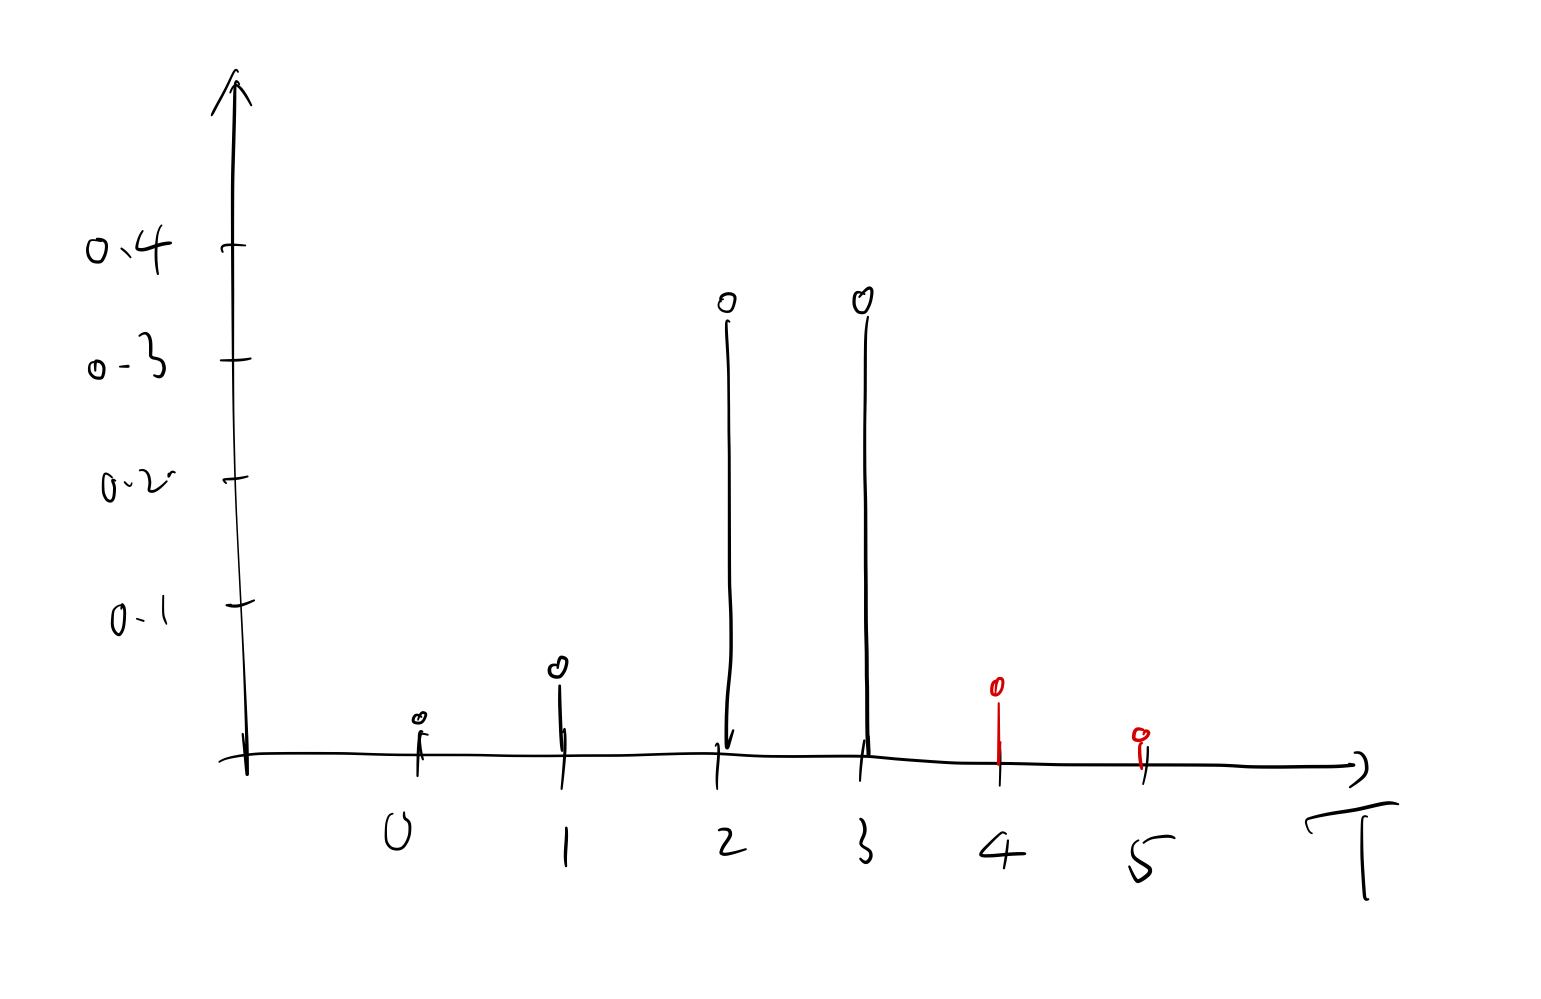
\includegraphics[width=0.7\textwidth]{figures/06-Hypothesis_testing/null_dist_binom.jpeg}
    %     \caption{猜拳實驗假說檢定的虛無分佈}
    %     \label{fig:}
    % \end{figure}

    % \begin{custom}{思考}
    %    如果把顯著水準提高,拒絕域應該會變寬或是變窄?
    % \end{custom}
    
    % \begin{table}[htbp]
    %     \begin{center}
    %         \begin{tabular}{ccccc}
    %             \toprule
    %             虛無假說($H_0$) & 對立假說($H_1$) & 檢定統計量 & $p$ 值 & 拒絕區\\
    %         \end{tabular}
    %         \caption{母體為常態分布且變異數未知的母體平均檢定\label{tab:}}
    %     \end{center}
    % \end{table}
    
    \bigskip 
    
    \begin{docexam}{(104-1醫學(一))}
        某研究為分析降血壓藥的效果,採用病例對照設計(case-control study),欲分析病例對照兩組樣本服降血壓藥3個月前後測量之血壓值差異是否有明顯不同,研究者應該使用何種統計方法最合適?

        (A) 配對 t 檢定 (Paired t-test)

        (B) 單一樣本 Z 檢定 (One sample Z-test)

        (C) Pearson 卡方檢定 (Pearson Chi-square test)

        (D) 獨立樣本 $t$ 檢定 (Independent t-test)
    \end{docexam}
    
    \begin{docexam}{(106-2醫學(二))}
        某研究者想檢定新藥是否有降血壓效果,對20隻大鼠在餵食新藥前後分別測量血壓值,對於兩次血壓測量值的比較,下列統計分析方法何者最恰當?

        (A) 線性回歸 (Linear regression)

        (B) 獨立樣本 $t$ 檢定 (Independent sample t-test)

        (C) 配對 t 檢定 (Paired t-test)

        (D) 列聯表分析 (Contingency table)
    \end{docexam}
    
    \begin{docexam}{(105-1醫學(一))}
        比較兩組病人某項檢驗數值的平均值(mean)是否有差異,可使用下列何種統計方法?

        (A) 卡方檢定 (Chi-square test)

        (B) $t$ 檢定 (Student's t test)

        (C) 曼惠特尼檢定 (Mann-Whitney test)

        (D) 符號檢定 (Sign test)
    \end{docexam}
    
    \begin{docexam}{(102-2醫學(一))}
        有關檢定兩個母群體平均值是否不同,統計推論可能會犯的錯誤型態及檢力 (power),下列何者錯誤?

        (A) 增加樣本數可以增加 power

        (B) 虛無假說為真時,作出推翻虛無假說的決定就犯 Type I error

        (C) 對立假說為真時,作出推翻虛無假說的決定的機率就是 power

        (D) 兩個母群體的平均值愈接近,power 就愈大
    \end{docexam}
    
    \begin{docexam}{(102-2醫學(一))}
        針對交通意外事故死亡者調查,從這些死亡者的左股動脈和左冠狀動脈各抽取血液樣本,以測量酒精濃度,總共抽取 25 個意外事故的死亡者。研究者的問題是「左股動脈的血液平均酒精濃度是否顯著不同於左冠狀動脈的血液平均酒精濃度?」你將採用何種統計方法檢定上述資料?

        (A) 獨立 $t$ 檢定

        (B) 卡方檢定

        (C) 配對 $t$ 檢定

        (D) 麥內瑪檢定 (McNemar's test)
    \end{docexam}
    
    \begin{docexam}{(101-2醫學(一))}
        有研究者報導其臨床試驗結果,實驗組的受試者感染率為 10\%,安慰劑組感染率為 13\%,兩組感染率差異的 95\% 信賴區間為 -2.6\% 至 8.6\%,下列敘述何者正確?        

        (A) 兩組的差異達統計顯著

        (B) 兩組的差異未達統計顯著

        (C) 應該採用變異數分析

        (D) 應該採用 $t$ 檢定
    \end{docexam}
    
    \begin{docexam}{(100-1醫學(一))}
        有一個研究探討某一藥物對於尿液鈣離子的排泄效應,有 9 位受試者被隨機選出,口服 0.5 毫克的藥物,在服用藥物 6 小時候收集這些人的尿液。另隨機抽取 16 位受試者,這些人不服用藥物,同樣在被隨機選出後 6 個小時收集這些人的尿液。研究者的問題是「這兩群人排泄的尿液鈣離子濃度是否顯著不同?」你將採用何種統計方法檢定上述資料?

        (A) 兩個樣本 $t$ 檢定

        (B) 卡方檢定

        (C) 配對 $t$ 檢定

        (D) 麥內瑪檢定 (McNemar's test)
    \end{docexam}
    
    \begin{docexam}{(110-1醫學(二))}
        如果想要比較年輕人與老年人的流感罹患率,王醫師隨機收集 $100$ 位年輕人與 $100$ 位老年人民眾,詢問其過去一個月是否罹患流感,其中有 $42$ 位年輕人及 $22$ 位老年人回答有,因此估計年輕人流感罹患率為 $0.42$,老年人流感罹患率為 $0.22$。下列何者最不恰當?

        (A) 王醫師的隨機抽樣必須排除有可能互相傳染的樣本,才能得到這些估計值

        (B) 王醫師的估計值 $0.42$,必須假設每個年輕人得流感的機率都是一樣且互相獨立,才能成立

        (C) 王醫師的老年人樣本如果源自 $1000$ 床的老人安養中心的隨機抽樣,則可能因為群聚效應,不宜視為獨立樣本

        (D) 王醫師可以合併樣本,利用 $200$ 人當中有 $42+22=64$ 位得到流感,來估計人口中得流感的機率為 $0.32$
    \end{docexam}

